\documentclass[french]{report}
\usepackage[utf8]{inputenc}
\usepackage[T1]{fontenc}
\usepackage{babel}
\usepackage{graphicx}
\usepackage{amsmath}
\usepackage{sectsty}
\usepackage{authblk}
\usepackage{algpseudocode}
\usepackage{algorithm}
\usepackage{xspace}
\usepackage{mathtools}
\usepackage{mathrsfs}
\usepackage{hyperref}
\documentclass[a4paper]{article}
\usepackage[T1]{fontenc}
\usepackage{textcomp}
%\usepackage[scaled]{beramono}
\usepackage{listings}
\usepackage{xcolor}
\usepackage{minted}
\usepackage[T1]{fontenc}
\usepackage{textcomp}
\usepackage[scaled]{beramono}
\newcommand{\HRule}{\rule{\linewidth}{0.5mm}}
\documentclass[12pt]{article}
\usepackage[francais]{babel}
\usepackage[T1]{fontenc}
\usepackage{listings}
 
\lstset{language=caml}
\providecommand{\keywords}[1]{\textbf{\textit{Keywords:}} #1}
\bibliographystyle{apalike}

\usepackage{hyperref}
\usepackage{fancyhdr} % entêtes et pieds de pages personnalisés

% définition de l'entête et du pied de page
\pagestyle{fancy}
\fancyhead[L]{PAP}
\fancyhead[R]{KOSSIR EL MEHDI  \& KARUNANAYAKGE SHAMAL}
\fancyfoot[C]{ \thepage}

\begin{document}

\begin{titlepage}

\begin{center}

\textsc{{\LARGE École Nationale Supérieure d'Informatique pour l'Industrie et l'Entreprise} \\ \vspace{6
    mm} {\Large ENSIIE}} \\
\vspace{5mm}
\includegraphics[width=0.4\textwidth]{./ENS}\\[1.0 cm]

\textsc{\Large   Projet C++}\\[0.5cm]

% Title
\HRule \\[0.4cm]
{ \huge \bfseries Equation de la chaleur}\\[0.4cm]

\HRule \\[1.5cm]
% Author and supervisor
\begin{minipage}{0.4\textwidth}
\begin{flushleft} \large
\emph{Authors:}\\
El Mehdi \textsc{Kossir} \\
{\small\href{mailto:prenom1.nom1@ensiie.fr}{elmehdi.kossir@ensiie.fr}}
\\
Shamal \textsc{Karunanayakage} \\
{\small\href{mailto:prenom2.nom2@ensiie.fr}{shamalmaduwantha.karunanayakage@ensiie.fr}}
\end{flushleft}
\end{minipage}
\begin{minipage}{0.4\textwidth}
\begin{flushright} \large
\emph{Encadrant :} \\
 \textsc{Vincent Torri} \\
    {\small\href{mailto:prenom1.nom1@ensiie.fr}{vincent.torri@gmail.com}}
\end{flushright}
\end{minipage}



% Date
\vfill
{\Large 16 Janvier 2021}
\end{center}
\end{titlepage} 




% New page
\begin{abstract}
Dans le cadre de l'UE << Programmation avancée et Projet>> . On a réalisé ce projet  en C++ qui s'intéresse à la résolutin numérique de l'équation de la chaleur en 1D et 2D.\\\\
L'objectif est de simuler l’évolution de la température dans un
matériau.\\\\
Ce phénomène de diffusion de la chaleur fut découvert et modélisé pour la première fois
en 1811, par le célèbre physicien et mathématicien Joseph Fourier. C'est à Grenoble qu'il
conduit ses expériences sur la propagation de la chaleur qui lui permettront de modéliser
l'évolution de la température au travers de séries trigonométriques (séries de Fourier). \\
Nous allons dans un premier temps  étudier la propagation de la chaleur dans \textbf{ une barre}(1D) Et après  dans \textbf{une plaque}(2D).\\\\

\small \textbf{Remarque : Vous trouverez l'implémentation de toutes les fonctions définies dans ce rapport ainsi que la documentation dans le ficher de code}.
\end{abstract}

% New page
\tableofcontents





% Chapitre 1
\chapter{Introduction }
Commençons par un petit point scientifique et parlons de l'équation de la chaleur. C'est une équation aux dérivées partielles parabolique qui a été introduite par Joseph Fourier en 1807. Elle décrit la conduction thermique c'est-à-dire qu'elle modélise la façon dont une quantité de chaleur se diffuse dans un environnement donné. \\ 
Cette équation définit par : 
\bigbreak
    $ \frac{\partial u(x,t)}{\partial t} =\frac{\lambda}{\rho c} \Delta u(x,t) + \frac{F}{\rho c}$
    \leftskip=3cm
\bigbreak
\leftskip = 0cm

avec u :  la température en degré K (Kelvin) en fonction du temps et de l'espace. \\
$\Delta$ le Laplacien sur  $[O,L]^{d}$ \\
F : $\mathbb {R}_{+} \times [O,L]^{d} \to \mathbb {R}_{+}$ la source de chaleur appliquée sous l’objet \\
$\lambda$ la conductivité thermique en W/(m.K)\\
$\rho$ la masse volumique en kg/m3\\
c la chaleur massique en J/(kg.K) \\

A travers ce sujet nous allons donc simuler l'évolution de la température dans deux cas différents :

\begin{itemize}
    \item Sur la barre \\
    C'est à dire un probleme unidimensionnel. 
    \item Sur la plaque \\
    C'est à dire un probleme de dimensions 2. \\
\end{itemize}

Pour chaque cas, on appliquera l'équation sur différents type de matériaux.

\begin{center}
   \begin{tabular}{| l | c | c | r |}
     \hline
      & $\lambda$ (W/(m.K)) & $\rho$ (kg/m3) & c (J/(kg.K))\\ \hline
     Cuivre & 389 & 8940 & 380 \\ \hline
     Fer & 80.2 & 7874 & 440 \\ \hline
     Verre & 1.2 & 2530 & 840 \\\hline
     Polystyrène & 0.1 & 1040 & 1200 \\
     \hline
   \end{tabular}
\end{center}
 
 
 
 
 
 

% Chapitre 2
\chapter{Méthodologie et organisation du travail }
Afin de gérer au mieux la gestion du projet et donc avoir un fonctionnement interne clair et propice à un  bon esprit d'équipe, nous avons utilisé différents logiciels.

\begin{itemize}
\item  \textbf{Git} \\
Il s'agit d'un logiciel de gestion de versions du code, qui créé différentes versions d'un projet au fur et à mesure que les fichiers sont édités.\\
Pour résumer, Git c'est tout simplement parfait pour manager les projets et évités des erreurs qui peuvent coûter très cher, par exemple en revenant sur des versions précédentes si besoin. On y gagne à la fois en temps et en qualités
\item \textbf{Discord} \\
Il s'agit d'un logiciel de VoIP gratuit. C'est un site sur lequel vous vous connectez pour discuter à l'oral ou à l'écrit tout en ayant la possibilité d'activer la webcam. Le partage d'écran est également disponible ce qui est pratique pour un projet en groupe, et notamment en cette période où la possibilité de se réunir pour travailler en groupe est plus compliqué.
\item \textbf{Trello} \\
Trello est un outil collaboratif conçu pour organiser ses tâches et gérer ses projets. Sous la forme d'une application web, Trello permet d'y voir plus clair dans la gestion de projet. \newline
\end{itemize} 

Les logiciels que nous avons utilisé pour réaliser ce projet sont :
\begin{itemize}
\item  \textbf{Visual Studio Code} \\
Il s'agit d'un éditeur de code extensible qui présente de multitude de fonctionnalités incluant la prise en charge du débogage, la mise en évidence de la syntaxe, la complétion intelligente du code ou encore  la refactorisation du code et Git intégré. 
\item \textbf{Scilab} \\
Il s'agit d'un logiciel libre de calcul numérique. Il contient quelques centaines de fonctions mathématiques, mais on peut aussi en ajouter de nouvelles via des programmes écrit en divers langages (C, C++, Java, etc.). On peut également créer des graphiques 2D/3D et des animations ce qui nous sera utile pour la réalisation de ce projet.\\\\

\end{itemize}


\begin{minipage}[c]{.46\linewidth}
     \begin{center}
           
             \includegraphics[width=7cm]{git.jpeg}
            
         \end{center}
   \end{minipage} \hfill
   \begin{minipage}[c]{.46\linewidth}
    \begin{center}
            \includegraphics[width=4cm]{discord.jpg}
        \end{center}
 \end{minipage}
 \bigbreak
 
 \begin{minipage}[c]{.46\linewidth}
     \begin{center}
           
             \includegraphics[width=7cm]{trello.png}
            
         \end{center}
   \end{minipage} \hfill
   \begin{minipage}[c]{.46\linewidth}
    \begin{center}
            \includegraphics[width=3cm]{vs.png}
        \end{center}
 \end{minipage}
 
 \begin{figure}[htbp] 
   \begin{center} 
      \includegraphics[width=7cm]{scilab.jpg} 
   \end{center} 
  
\end{figure} \\




% Chapitre 3
\chapter{Travaux réalisés }
Comme on l'a vu dans l'introduction, l’équation aux dérivées partielles simulant la propagation de la
chaleur s’appelle (à juste titre) l’équation de la chaleur dans le cas unidimensionnel cette équation est définit par :\bigbreak
    $ \frac{\partial u(x,t)}{\partial t} =\frac{\lambda}{pc} \frac{\partial^2 u(x,t)}{\partial^2 x} + \frac{F}{pc}$
    \leftskip=3cm
\bigbreak
\leftskip = 0cm
Les quantités $\lambda$, p et c sont des grandeurs physiques, respectivement la conductivité thermique, la
masse volumique et la chaleur massique du matériau constituant l’objet.\\\\
\section{Équation de la chaleur : cas unidimensionnel (la barre)} 
\textbf{1er cas : La barre}\\\\
L’équation devient :
\bigbreak
$\begin{cases}
\frac{\partial u(x,t)}{\partial t} =\frac{\lambda}{pc} \frac{\partial^2 u(x,t)}{\partial^2 x} + \frac{F}{pc} &\forall(t,x) \in [0,tmax]*[0,L] \\
u(0,x) = u_0 &\forall(x) \in [0,L]
\\
\frac{\partial u(t,0)}{\partial x} = 0, &\forall(t) \in [0,tmax]
\\
u(t,L)=u_0, &\forall(t) \in [0,tmax]
\end{cases}$
\leftskip=3cm
\bigbreak
\leftskip = 0cm 

La source de chaleur F simule deux ajouts de chaleur,
de température f et $\frac{3}{4}f$, on respecte aussi les conditions au bord(Dirichlet, Neumann).\\\\

Il est impossible dans la plupart des cas de résoudre cette équation.. On recourt alors à la méthode des différences finies. 

On commence donc par réaliser une discrétisation en temps et en espace du problème en utilisant dans un premier temps car elle est plus facile et ça nou permettra d'avoir un comparatif \textbf{la méthode d'Euler explicite}.\\\\
\textbf{Discrétisation du terme $\frac{\partial u(x,t)}{\partial t}$}:\\\\
On impose un pas constant :\\
$\forall(i), t_{i+1} - t{i} = \tau$ \\
$\forall(n), x_{n+1} - x_{n} = h $ \\\\
Soit le développement de Taylor à l'ordre 1 :\\

$u(x,t_{i+1})=u(x,t_{i}+\tau)$ on a $\tau << 1$ donc 
$u(x,t_{i+1}) \approx u(x,t_{i}) +\tau \frac{\partial u(x,t)}{\partial t}|_{t=t_i} + O(\tau^2) $\\\\
Donc 
$\frac{\partial u(x,t)}{\partial t}|_{t=t_i} \approx \frac{u(x_n,t_{i+1})-u(x_n,t_{i})}{\tau} \approx \frac{u_n^{i+1}-u_n^{i}}{\tau}$\\\\
\textbf{Discrétisation du terme $\frac{\partial^2 u(x,t)}{\partial^2 x}$}:\\\\
Soit le développement de Taylor à l'ordre 2 :\\
$u(x_{n+1},t)=u(x_{n}+h,t)$ on a $h << 1$ donc 
$u(x_{n+1},t) \approx u(x_{n},t) +h \frac{\partial u(x,t)}{\partial x}|_{x=x_n}+\frac{h}{2!}\frac{\partial^2 u(x,t)}{\partial^2 x}|_{x=x_n} + O(h^3) $\\\\
Donc 
$\frac{\partial^2 u(x,t)}{\partial^2 x}|_{x=x_n} \approx \frac{u_{n+1}^{i}+u_{n-1}^{i} -2u_{n}^{i} }{h^2}$\\\\
On remplace dans l'équation 1 :\\\\
$pc (\frac{u_n^{i+1}-u_n^{i}}{\tau}) = \lambda(\frac{u_{n+1}^{i}+u_{n-1}^{i} -2u_{n}^{i} }{h^2}) +F$\\\\
On pose $a=\frac{\lambda}{pc} *\frac{\tau}{h}$ \\\\
On trouve alors l'équation discrétiser du problème : \\\\
$u_n^{i+1} =  a u_{n-1}^{i} + (1-2a)u_{n}^{i} +au_{n+1}^{i} +\frac{ah^2}{\lambda}F $\\\\
avec :\bigbreak
$ u(0,x) = u_0 ,
\frac{\partial u(t,0)}{\partial x} = 0, 
u(t,L)=u_0.$\\\\
\textbf{Méthode d'Euler implicite :}\\\\
Nous utilisons un schéma arrière d'ordre 1 pour évaluer la dérivée temporelle et un schéma centré
d'ordre 2 pour la dérivée seconde en espace :\\

$\frac{\partial u(x,t)}{\partial t}|_{t=i+1} \approx \frac{u_{n}^{i+1}-u_n^{i}}{\tau}$\\

$\frac{\partial^2 u(x,t)}{\partial^2 x} \approx \frac{u_{n+1}^{i+1}+u_{n-1}^{i+1} -2u_{n}^{i+1} }{h^2}$\\\\
En posant $a= \frac{\frac{\lambda}{pc}\tau}{h^2}$
, la température à l'itération i + 1 est donnée par :\\

$u_n^{i} =(1+2a)u_n^{i+1} - a(u_{n+1}^{i+1} + u_{i+1}^{n-1}) -\frac{\tau F}{pc}$:  n variant de 1 à N-1 avec N+1 le nombre de noeuds de coordonées $x_n$

On peut écrire cette équation sous forme matricielle :

$$
\begin{bmatrix}
   1+2a & -a  & 0& \cdots & 0\\
   -a & 1+2a & -a& \cdots& 0\\
   \vdots & \ddots & \ddots & \ddots & \vdots \\
    0 & \cdots& -a & 1+2a & -a \\
    0 & \cdots & 0 & -a & 1+2a \\
\end{bmatrix}
\begin{bmatrix}
    u_{1}\\
    u_{2}\\
    \vdots\\
    u_{N-1}\\
\end{bmatrix}^{i+1}
=
\begin{bmatrix}
    u_{1}\\
    u_{2}\\
    \vdots\\
    u_{N-1}\\

\end{bmatrix}^{i}
+a
\begin{bmatrix}
    u0\\
    0\\
    \vdots\\
    0\\
    u0\\
\end{bmatrix}^{i}
+\frac{ \tau F}{p c}
$$\\
\textbf{Résolution par la méthode de cholesky :}\\\\
L'équation discrétiser peut s'écrire sous la forme: $AT=b$, on remarque que la matrice A est une matrice tridiagonale, la matrice A peut se decomposer sous la forme $A = LU$, avec les matrices

$$
L=
\begin{bmatrix}
   b_1* & 0 & 0& \cdots & 0\\
   -a & b_2* & & \cdots& 0\\
   \vdots & \ddots & \ddots & \ddots & \vdots \\
    0 & \cdots& -a & b_{n-1}* &  \\
    0 & \cdots & 0 & -a & b_{n}* \\
\end{bmatrix}\\
U=
\begin{bmatrix}
   1 & c_1* &0 & \cdots & 0\\
   0 & 1 & & \cdots& 0\\
   \vdots & \ddots & \ddots & \ddots & \vdots \\
    0 & \cdots& 0& 1 & c_{n-1}*& \\
    0 & \cdots & 0 & 0 & 1\\
\end{bmatrix}\\
$$ avec : \\

$\begin{cases}
b_1* =b_1  , b_k^* =b_k - a*c_{k-1}^*\\\
c_1* =\frac{c_1}{b_1}  ,  c_k^* =c_k/b_k*\\

\end{cases}$\\\\\\
Le système peut être résolu maintenant en deux etapes  $AT \Leftrightarrow   LUT=F$ avec $UT=Y$.(voir méthode (à remplir) dans le fichier du code)


\section{Équation de la chaleur  : cas 2 dimensions (la plaque)}

Nous souhaitons à présent pouvoir résoudre l’équation de la chaleur en 2D.

\textbf{2ème cas : La plaque}\\\\

L’équation devient :
\bigbreak
$\begin{cases}
\frac{\partial u}{\partial t} =\frac{\lambda}{pc}( \frac{\partial^2 u}{\partial^2 x}+\frac{\partial^2u}{\partial^2 y}) + \frac{F}{pc} &\forall(t,x,y) \in [0,tmax]*[0,L]^2 \\
u(0,x,y) = u_0 &\forall(x,y) \in [0,L]^2
\\
\frac{\partial u(t,0,y)}{\partial x} = 0, &\forall(t,y) \in [0,tmax] * [0,L]
\\
\frac{\partial u(t,x,0)}{\partial y} = 0, &\forall(t,x) \in [0,tmax] * [0,L]
\\
u(t,L,y)=u_0, &\forall(t,y) \in [0,tmax]*[0,L]
\\
u(t,x,L)=u_0, &\forall(t,x) \in [0,tmax]*[0,L]
\end{cases}$
\leftskip=3cm
\bigbreak
\leftskip = 0cm
\\
Comme dans le cas 1D, On impose un pas constant :\\\\
$\forall(i), t_{i+1} - t{i} = \tau$ \\
$\forall(n), x_{n+1} - x_{n} = h_x $ \\
$\forall(j), y_{j+1} - y_{j} = h_y $ \\\\
On a par la méthode d'Euler implicite :\\\\
$\frac{\partial u(x,y,t)}{\partial t}|_{t=t_i} \approx \frac{u(x_n,y_j,t_{i+1})-u(x_n,y_j,t_{i})}{\tau} \approx \frac{u_{n,j}^{i+1}-u_{n,j}^{i}}{\tau}$\\\\
$\frac{\partial^2 u(x,y,t)}{\partial^2 x} \approx \frac{u_{n+1,j}^{i+1}+u_{n-1,j}^{i+1} -2u_{n,j}^{i+1} }{h_x^2}$\\\\
$\frac{\partial^2 u(x,y,t)}{\partial^2 y} \approx \frac{u_{n,j+1}^{i+1}+u_{n,j-1}^{i+1} -2u_{n,j}^{i+1} }{h_y^2}$\\\\
On remplace dans l'équation 1 :\\\\
$pc (\frac{u_{n,j}^{i+1}-u_{n,j}^{i}}{\tau}) = \lambda(\frac{u_{n+1,j}^{i+1}+u_{n-1,j}^{i+1} -2u_{n,j}^{i+1} }{h_x^2} + \frac{u_{n,j+1}^{i+1}+u_{n,j-1}^{i+1} -2u_{n,j}^{i+1} }{h_y^2}) +F$ donc :\\\\ 
$u_{n,j}^{i}=u_{n,j}^{i+1}(1+\frac{2\lambda*\tau}{\rho c h_x^2}+\frac{2\lambda*\tau}{\rho c h_y^2})-\frac{\tau\lambda}{\rho c}(\frac{u_{n+1,j}^{i+1}+u_{n-1,j}^{i+1}  }{h_x^2}+\frac{u_{n,j+1}^{i+1}+u_{n,j-1}^{i+1}  }{h_y^2}) $\\\\
On pose $\sigma =\frac{\lambda}{\rho c}$ et on définit H la matrice du laplacien 2D par :\\\\

$$
H=
\begin{bmatrix}
   \frac{2}{h_x^2}+\frac{2}{h_y^2} & \frac{-1}{h_x^2} &\cdots &\frac{-1}{h_y^2} &\cdots & 0\\
   \frac{-1}{h_x^2}  & \frac{2}{h_x^2}+\frac{2}{h_y^2} & \frac{-1}{h_x^2}&\cdots& \frac{-1}{h_y^2}&\cdots& \\
   \vdots & \ddots & \ddots & \ddots & \vdots \\
    0 & \cdots& \frac{2}{h_x^2}+\frac{2}{h_y^2} & -\frac{IdN_x}{h_y^2} &  \\
    0 & \cdots & -\frac{IdN_x}{h_y^2} & \frac{2}{h_x^2}+\frac{2}{h_y^2} &  \\
\end{bmatrix}\\
$$

Le problème se réecrit alors : 
$U^{n+1} =U^{n} + \tau(-\sigmaH +\frac{F^n}{\rho c} )$.











% Chapitre 4
\chapter{Conception}
Nous avons  précédemment vu la résolution de l'équation de la chaleur dans son aspect mathématiques. Informatiquement, une représentation de l'équation de la chaleur est possible. On se basera sur le diagramme UML suivant pour notre conception.
\section{Diagramme UML :}

\begin{figure}[htbp] 
   \begin{center} 
      \includegraphics[width=8cm]{DiagrammeUml.png} 
   \end{center} 
   \caption{\footnotesize Diagramme UML} 
\end{figure} \\

Après avoir établi les formules de calcul du u(x,t) propres aux deux méthodes employées (1D, 2D).\\ \\
On a appliqué notre code sur les différents matériaux ci dessous :

\begin{center}
    \begin{tabular}{|c|c|l|r|} 
        \hline  
        &\lambda &\rho &c \\  
        \hline 
        cuivre & 389 & 8940 & 380 \\  
        \hline 
        fer & 80.2 & 7874 & 440\\ 
        \hline 
        verre & 1.2 & 2530 & 840\\ 
        \hline 
        polystyrène & 0.1 & 1040 & 1200\\ 
        \hline
    \end{tabular} 
\end{center}

Pour tous les matériaux on a écrit dans un fichier les valeurs de la solution approchée sous forme de colonne, ensuite on l'a utilisé dans le programme Scilab pour avoir une animation de la solution approchée de $u(t, .)$ pour 100 valeurs de t réparties uniformément sur [0, tmax].

\section{Résultats 1er cas : La barre}
\subsection{Cuivre} 

\begin{minipage}[c]{.46\linewidth}
     \begin{center}
           
             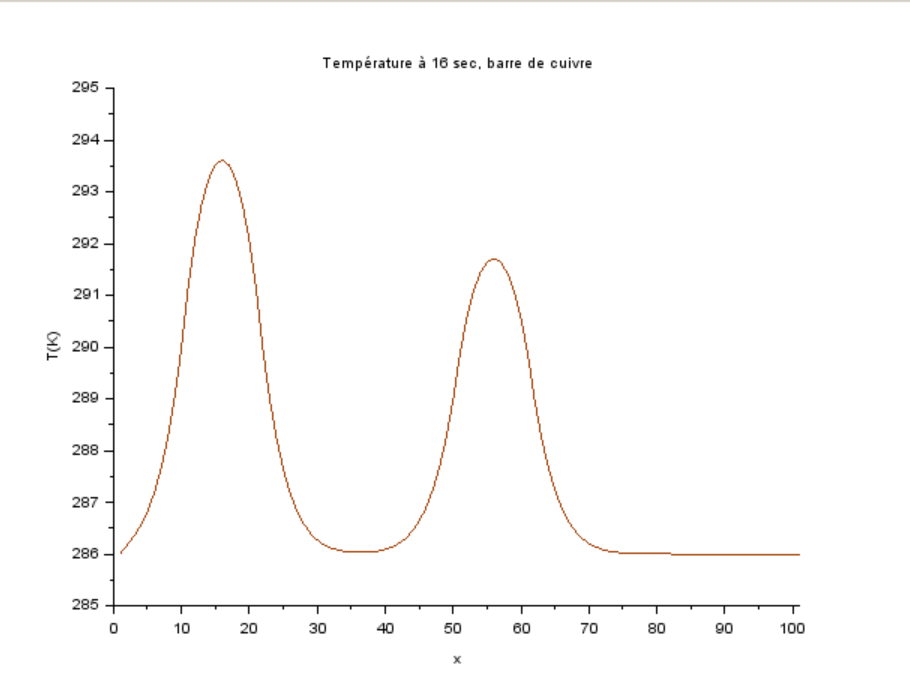
\includegraphics[width=7cm]{C.png}
            
         \end{center}
   \end{minipage} \hfill
   \begin{minipage}[c]{.46\linewidth}
    \begin{center}
            \includegraphics[width=7cm]{C8.png}
        \end{center}
 \end{minipage}

\subsection{Verre}
\begin{minipage}[c]{.46\linewidth}
     \begin{center}
             \includegraphics[width=7cm]{V.png}
         \end{center}
   \end{minipage} \hfill
   \begin{minipage}[c]{.46\linewidth}
    \begin{center}
            \includegraphics[width=7cm]{V8.png}
        \end{center}
 \end{minipage}
 
 \subsection{Fer}
\begin{minipage}[c]{.46\linewidth}
     \begin{center}
             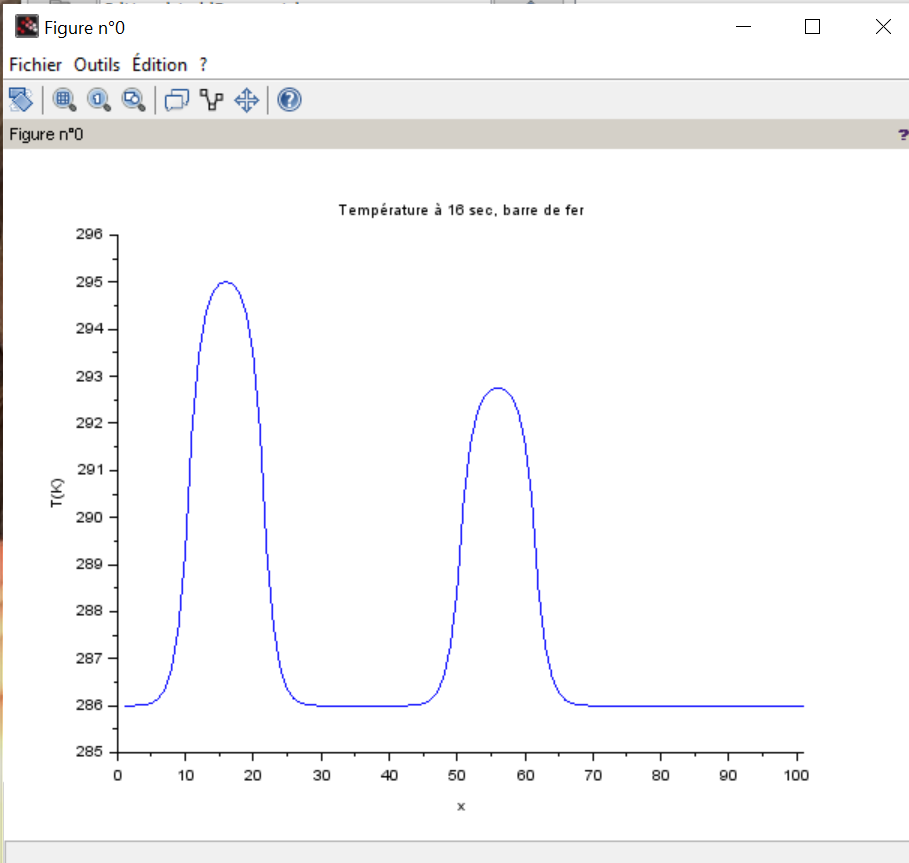
\includegraphics[width=7cm]{fer.png}
         \end{center}
   \end{minipage} \hfill
   \begin{minipage}[c]{.46\linewidth}
    \begin{center}
            \includegraphics[width=7cm]{fer8.png}
        \end{center}
 \end{minipage}
 
  \subsection{Polystyrène}
\begin{minipage}[c]{.46\linewidth}
     \begin{center}
             \includegraphics[width=7cm]{P.png}
         \end{center}
   \end{minipage} \hfill
   \begin{minipage}[c]{.46\linewidth}
    \begin{center}
            \includegraphics[width=7cm]{P8.png}
        \end{center}
 \end{minipage}\\\\\\
 
 \newpage
 \section{Résultats 2ème cas : La plaque}
\subsection{Cuivre}

\begin{figure}[htbp] 
   \begin{center} 
      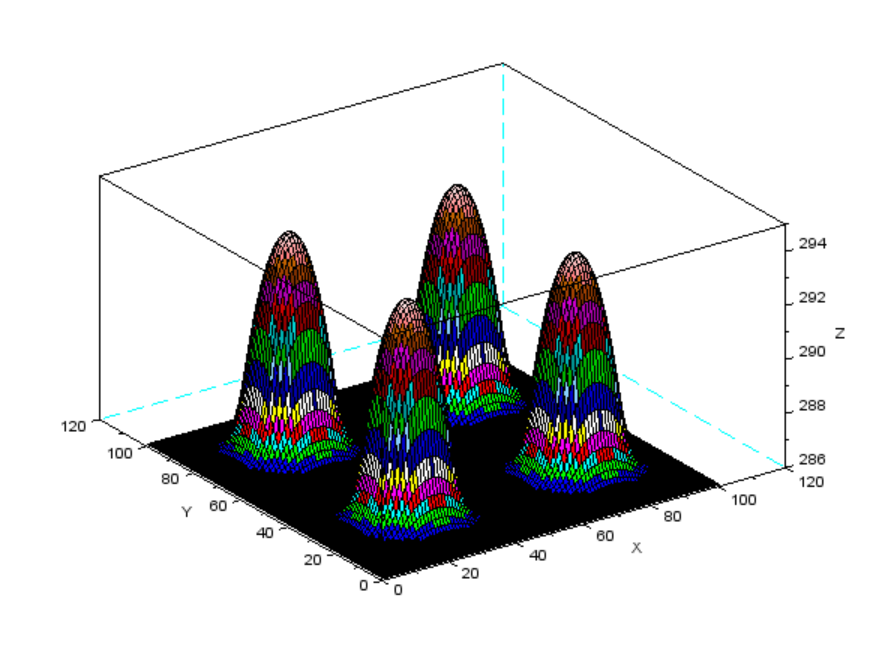
\includegraphics[width=7cm]{cuivre2D.PNG} 
   \end{center} 
   \caption{\footnotesize Plaque de cuivre} 
\end{figure} \\
\subsection{Verre}
\begin{figure}[htbp] 
   \begin{center} 
      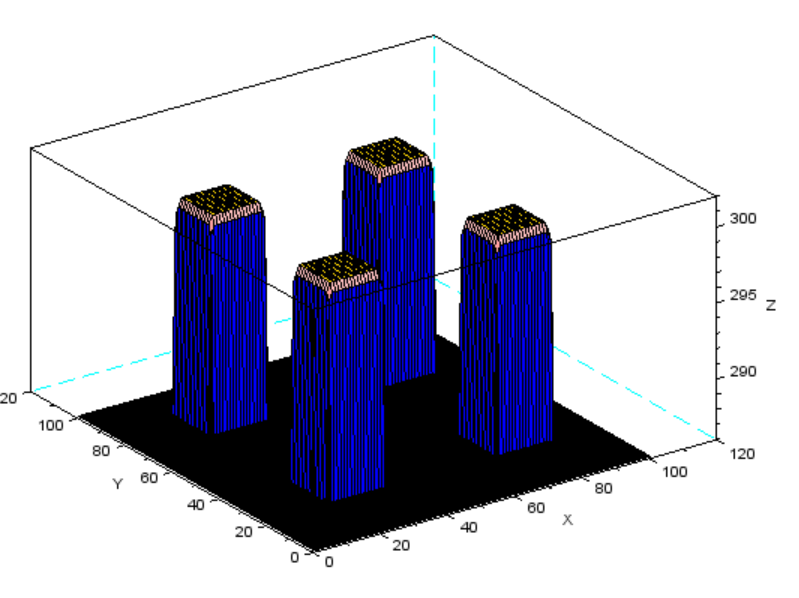
\includegraphics[width=7cm]{verre2d.PNG} 
   \end{center} 
   \caption{\footnotesize Plaque de verre} 
\end{figure} \\\\\\
\subsection{Fer}
\begin{figure}[htbp] 
   \begin{center} 
      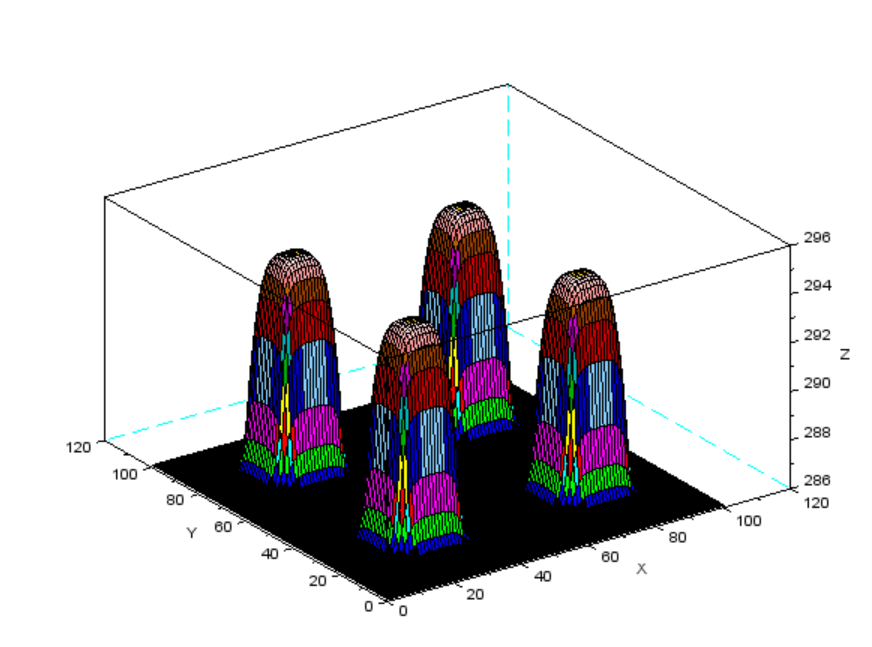
\includegraphics[width=7cm]{fer2d.PNG} 
   \end{center} 
   \caption{\footnotesize Plaque de fer} 
\end{figure} \\\\\
\subsection{Polystyrène}
\begin{figure}[htbp] 
   \begin{center} 
      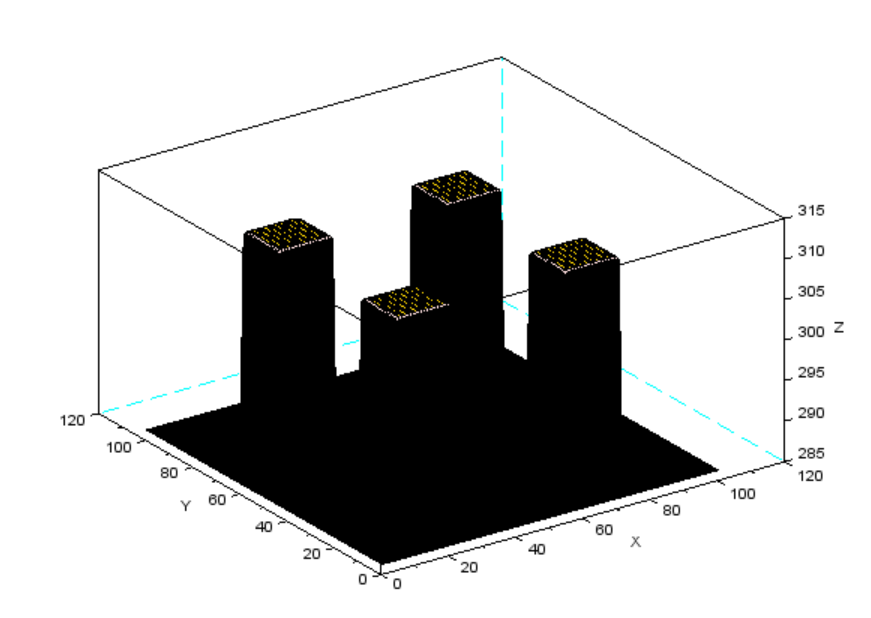
\includegraphics[width=7cm]{po2d.PNG} 
   \end{center} 
   \caption{\footnotesize Plaque de polystyrène} 
\end{figure} \\

\subsection{Commentaires}\\

On observe  que plus la diffusivité thermique $\frac{\lambda}{\rho c}$ est grande 
plus la chaleur se répartie dans le matériaux.\\

On voit aussi que plus ce coefficient est faible, plus la température augmente aux points d’application de la source de chaleur.\\

% Chapitre 5
    \chapter{Problèmes rencontrées}
La partie, consistant à reformuler
informatiquement les formules mathématiques, fut la plus délicate car la moindre
erreur dans les paramètres de la boucle entraînait un effet boule de neige sur la suite du
programme en créant davantage de termes que ceux voulus ou en renvoyant des valeurs
erronées en certains points.\\
    Ainsi des incrémentations se trouvèrent
    défaillantes dans notre programme entraînant la
présence d'une dizaine de valeurs nulles pour l'une des fonctions calculées. De même,
lorsque la boucle se prolongeait jusqu'à n+1 au lieu de s'arrêter à n, le nombre de valeurs
obtenues se trouvait être faux. Enfin si cette erreur n'était pas une erreur de syntaxe, elle n'était pas détectée lors de la compilation du programme ce qui compliquait davantage sa détection et faisait perdre beaucoup de temps dans l'avancement du programmation.



% Chapitre 6
\chapter{Conclusion}

Ce projet s’est révélé très enrichissant dans la mesure où il a consisté en une approche concrète du métier d’ingénieur. En effet, la prise d’initiative, le respect des délais et le travail en équipe seront des aspects essentiels de notre futur métier. 
De plus il nous a permis de stimuler notre créativité et de trouver des idées originales que nous avons essayé de mettre en œuvre.\\

De plus, le fait que le choix du thème du projet soit libre, cela nous a permis de nous pencher sur une question qui nous intéressait fortement. \\

Ce rapport fut aussi bénéfique car il nous a permis d'apprendre de nouvelles choses ainsi que d'approfondir nos connaissances en C++, et cela en mettant en oeuvre ce que l'on a vu en UE de programmation avancée et projet. 


% Chapitre 7
\chapter{Bibliographie}


\begin{itemize}
    \item https://fr.wikipedia.org/wiki/equationdelachaleur. \\\\

    \item web2.uqat.ca/lerene/Webcours/gen-0135/manuel/m41-0135.pdf. \\\\
    
    \item  http://www.siteduzero.com/. \\\\
    
    \item http://perso.ensc-rennes.fr/jimmy.roussel/apprendre/laplace/index.html.\\\\
    
    \item http://web2.uqat.ca/lerene/Webcours/gen-0135/manuel/m41-0135.pdf
    

\end{itemize}


\end{document}
